\documentclass{article}
\usepackage{amssymb}
\usepackage{amsmath}
\textheight20cm 

\usepackage[dvips]{color}
\usepackage{amsfonts}
\usepackage{graphicx}
\usepackage{latexsym}
\usepackage{rotating}
\usepackage{url}

\newcommand{\Q}{{\mathbb Q}}
\newcommand{\OO}{{\mathbb O}}
\newcommand{\Z}{{\mathbb Z}}
\newcommand{\R}{{\mathbb R}}
\newcommand{\N}{{\mathbb N}}
\newcommand{\X}{{\mathbb X}}

\setlength{\parindent}{0pt}
\setlength{\parskip}{2ex plus 0.4ex minus 0.4ex}

\title{A User's Guide for {\tt LattE} v1.1 \\ (Linux Release)
\footnote{Research supported by NSF grants DMS-0309694, NSF grants
DMS-0073815, and by NSF VIGRE Grant DMS-0135345. $\copyright$ 
Department of Mathematics, University of California, Davis, 2003. This
software is released under the GNU license agreement}}

\author{Jes\'us A. De Loera \and
        David Haws \and
        Raymond Hemmecke \and
        Peter Huggins \and 
        Jeremy Tauzer \and 
        Ruriko Yoshida }
\date{December 2003}

\begin{document}

\maketitle{}

\newpage

\tableofcontents

\newpage

\section{Introduction}

\subsection{What is {\tt LattE}?} \label{intro}

The name ``{\tt LattE}'' is an abbreviation for ``{\bf Latt}ice point 
{\bf E}numeration.'' So what exactly does {\tt LattE} do? The 
software's main function is to count the lattice points contained in 
convex polyhedra defined by linear equations and inequalities with 
integer coefficients. The polyhedra can be of any (reasonably small) 
dimension, and {\tt LattE} uses an algorithm that runs in polynomial
time for fixed dimension: Barvinok's algorithm \cite{BarviPom}. To
learn more about the exact details of our implementation and
algorithmic techniques involved, the interested reader can consult 
\cite{latte1,latte2,latte3} and the references listed therein. Here we
give a rather short description of the mathematical objects used by
{\tt LattE}, {\bf Barvinok's Rational Functions}:

\noindent
Given a convex polyhedron $P = \{u\in\R^d:Au\leq b\}$, where $A$ and
$b$ are integral, the fundamental object that we compute is a short 
representation of the infinite power series:
\[
f(P;x) \quad = \sum_{\alpha\in P\cap\Z^d} x_1^{\alpha_1}
x_2^{\alpha_2} \ldots x_d^{\alpha_d}.
\]
Here each lattice point is given by one monomial. Note that this can be 
a rather long sum, in fact for a polyhedral cone it can be infinite, but 
the good news is that it admits short representations.

\noindent {\bf Example:} Let $P$ be the quadrangle with vertices 
$V_1=(0,0)$, $V_2=(5,0)$, $V_3=(4,2)$, and $V_4=(0,2)$. 

\begin{figure}[thb]
\begin{center}
     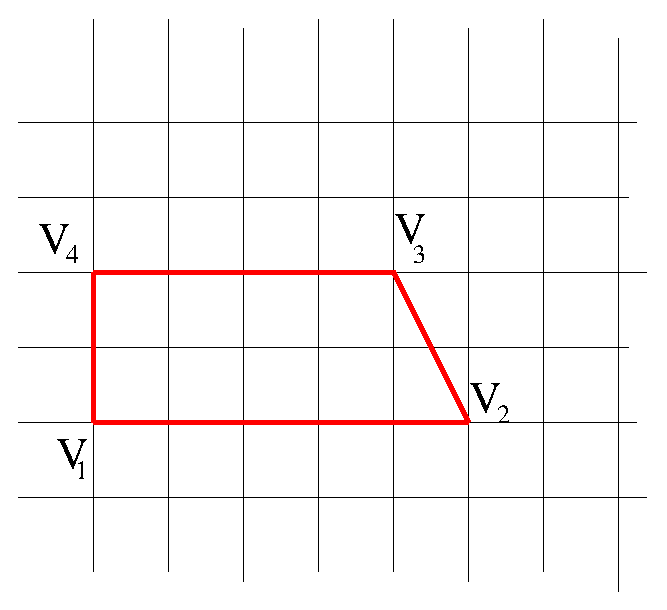
\includegraphics[scale=.79]{examplebrion.eps}
\end{center}
\end{figure}

{\small
\noindent
$f(P;x,y)={x}^{5}+{x}^{4}y+{x}^{4}+{x}^{4}{y}^{2}+y{x}^{3}+{x}^{3}+
{x}^{3}{y}^{2}+y{x}^{2}+{x}^{2}+{x}^{2}{y}^{2}+xy+x+x{y}^{2}+y+1+
{y}^{2}$
}

The fundamental theorem of Barvinok (circa 1993, see \cite{BarviPom})
says that you can write $f(P;x)$ as a sum of short rational functions,
in polynomial time when the dimension of the polyhedron is fixed.
In our running example we easily see that the 16 monomial polynomial
can be written as shorter rational function sum:

\noindent $f(P;x,y)=f(K_{V_1};x,y)+f(K_{V_2};x,y)+f(K_{V_3};x,y)+f(K_{V_4};x,y)$ 

\noindent where 

$f(K_{V_1};x,y)={\frac {1}{\left (1-x\right )\left (1-y\right )}} \quad f(K_{V_2};x,y)=\frac{({x}^{5}+{x}^{4}y)}{ (1-{x}^{-1}) (1-y^2x^{-1})}$

$f(K_{V_3};x,y)=\frac{({x}^{4}{y}^{2}+{x}^{4})}{ (1-{x}^{-1})
(1-xy^{-2})}
 \quad  f(K_{V_4};x,y)=\frac{y^{2}}{(1-{y}^{-1} )(1-x )}$
\vskip .5cm

$ f(P; 1,1)=16$

Counting the lattice points in convex polyhedra is a powerful tool which 
allows many applications in areas such as Combinatorics, Statistics, 
Optimization, and Number Theory. 

\subsection{What can {\tt LattE} compute?}

In the following we list the operations that {\tt LattE} v1.1 can
perform on bounded convex polyhedra (more commonly referred to as 
\textit{polytopes}). For the reader's convenience, we already include
the basic commands to actually do the tasks. Let us assume that a
description of a polytope $P$ is given in the file ``fileName'' (see
Section \ref{Input Files} for format) and that a cost vector is
specified in the file ``fileName.cost'' (needed for the optimization
part, see Section \ref{Input Files} for format).

Tasks performed by {\tt LattE} v1.1:
\begin{enumerate}
\item Count the number of lattice points in $P$.
\begin{verbatim}
     ./count fileName
\end{verbatim} 
\item Count the number of lattice points in $nP$, the dilation of $P$
  by the integer factor $n$.
\begin{verbatim}
     ./count dil n fileName
\end{verbatim} 
\item Calculate a rational function that encodes the \textit{Ehrhart
  series} associated with the polytope. By definition, the $n$-th
  coefficient in the Ehrhart series equals the number of lattice
  points in $nP$. For more details on Ehrhart counting functions see,
  for example, Chapter 4 of \cite{stanley}. 
\begin{verbatim}
     ./ehrhart fileName
\end{verbatim} 
\item Calculate the first $n+1$ terms of the Ehrhart series associated
  with the polytope.  
\begin{verbatim}
     ./ehrhart n fileName
\end{verbatim} 
\item Maximize or minimize a given linear function of the lattice
  points in $P$.
\begin{verbatim}
     ./maximize fileName
     ./minimize fileName
\end{verbatim} 
\end{enumerate}	

In addition to these basic functions, there are more specific calls to
{\tt LattE}. For example to use the homogenized Barvinok algorithm
instead of the original one in order to count the lattice points. These
details will be explained in Section \ref{Running LattE}.



\newpage

\section{Downloading and Installing {\tt LattE}}

{\tt LattE} is downloadable from the following website:

\makebox[12 cm]{http://www.math.ucdavis.edu/$\sim$latte/downloads/}

\textbf{Step 1: Create directory for {\tt LattE}}

\begin{verbatim}
     mkdir latte
\end{verbatim}

\textbf{Step 2: Download ``latte\_v1.1.tar.gz'' to directory ``latte''}

\begin{verbatim}
     Download ``latte_v1.1.tar.gz'' from
\end{verbatim}

\makebox[12 cm]{http://www.math.ucdavis.edu/$\sim$latte/downloads/}
 
(If you have never downloaded a file from the internet: A click with
your right mouse button onto the file name on the webpage should do
the trick. In any case, if you do not succeed, ask your system
administrator, a friend, or send us an email.) 

\textbf{Step 3: Change to directory for ``latte''}

\begin{verbatim}
     cd latte
\end{verbatim}

\textbf{Step 4: Unzip and untar the archive} 

\begin{verbatim}
     gunzip latte_v1.1.tar.gz
     tar xvf latte_v1.1.tar
\end{verbatim}

\textbf{Step 5: Make ``install'' executable} 

\begin{verbatim}
     chmod 700 install
\end{verbatim}

\textbf{Step 6: Install {\tt LattE}} 

\begin{verbatim}
     ./install
\end{verbatim}



\newpage

\section{Input Files}\label{Input Files}

\subsection{{\tt LattE} Input Files}

\subsubsection{Inequality Description}
For computations involving a polytope $P$ described by a
system of inequalities $Ax\leq b$, where $A\in\Z^{m\times d}$, 
$A=(a_{ij})$, and $b\in\Z^m$, the {\tt LattE} readable input file
would be as follows: 
\begin{verbatim}
m d+1
b  -A
\end{verbatim}

\textbf{EXAMPLE.}
Let $P=\{(x,y): x\leq 1, y\leq 1, x+y\leq 1, x\geq 0, y\geq 0\}$.
Thus
\[
\begin{array}{ccc}
A=\left(
\begin{array}{rr} 
 1 &  0 \\ 
 0 &  1 \\ 
 1 &  1 \\
-1 &  0 \\ 
 0 & -1 \\ 
\end{array} 
\right) 
& , &
b = \left( 
\begin{array}{r} 
1 \\ 
1 \\ 
1 \\ 
0 \\
0 \\ 
\end{array} 
\right)
\end{array}
\]
and the {\tt LattE} input file would be as such:
\begin{verbatim}
5 3
1 -1  0
1  0 -1
1 -1 -1
0  1  0
0  0  1
\end{verbatim}

\subsubsection{Equations}
In {\tt LattE}, polytopes are represented by {\bf linear constraints},
i.e. equalities or inequalities. By default a constraint is an
inequality of type $ax\leq b$ unless we specify, by using a single
additional line, the line numbers of constraints that are linear
equalities. 

\textbf{EXAMPLE.}
Let $P$ be as in the previous example, but require $x+y=1$ instead of
$x+y\leq 1$, thus, 
$P=\{(x,y): x\leq 1, y\leq 1, x+y=1, x\geq 0, y\geq 0\}$.
Then the {\tt LattE} input file that describes $P$ would be as such:
\begin{verbatim}
5  3
1 -1  0
1  0 -1
1 -1 -1
0  1  0
0  0  1
linearity 1 3
\end{verbatim}
The last line states that among the $5$ inequalities one is to be
considered an equality, the third one.

\subsubsection{Nonnegativity Constraints}
For bigger examples it quickly becomes cumbersome to state all
nonnegativity constraints for the variables one by one. Instead, you
may use another short-hand.

\textbf{EXAMPLE.}
Let $P$ be as in the previous example, then the {\tt LattE} input file
that describes $P$ could also be described as such: 
\begin{verbatim}
3  3
1 -1  0
1  0 -1
1 -1 -1
linearity 1 3
nonnegative 2 1 2
\end{verbatim}
The last line states that there are two nonnegativity constraints and
that the first and second variables are required to be nonnegative. 
{\bf NOTE} that the first line reads ``3 3'' and not ``5 3'' as above! 

\subsubsection{Cost Vector}
The functions maximize and minimize solve the integer linear programs
\[
\max\{c^\intercal x: x\in P\cap\Z^d\}
\]
and
\[
\min\{c^\intercal x: x\in P\cap\Z^d\}.
\]
Besides a description of the polyhedron $P$, these functions need a
linear objective function given by a certain cost vector $c$. If the
polyhedron is given in the file ``fileName''
\begin{verbatim}
4  4
1 -1  0  0
1  0 -1  0
1  0  0 -1
1 -1 -1 -1
linearity 1 4
nonnegative 3 1 2 3
\end{verbatim}
the cost vector must be given in the file ``fileName.cost'', as for
example in the following three-dimensional problem: 
\begin{verbatim}
1 3
2 4 7
\end{verbatim}
The first two entries state the size of a $1\times n$ matrix (encoding
the cost vector), followed by the $1\times n$ matrix itself. Assuming
that we call maximize, this whole data encodes the integer program
\[
\max\{2x_1+4x_2+7x_3: x_1+x_2+x_3=1, x_1,x_2,x_3\in\{0,1\}\}.
\]



\subsection{{\tt cdd} Input Files}
In addition to the formats described above, {\tt LattE} can also
accept input files in standard {\tt cdd} format. (See Subsection 
\ref{Command Syntax} for
details on how to run {\tt LattE} on a {\tt cdd} input file.) Below is
an example of {\tt cdd} input that is readable into {\tt LattE}.
\begin{verbatim}
H-representation
begin
4  4  integer
2 -2  4 -1
3 -2 -2  3
6  2 -4 -3
1  2  2  1
end
\end{verbatim}
It is important to note that {\tt LattE} can only read 
{\em integer} input.  Clearly, {\tt cdd}'s rational data files can be
converted into integer files by multiplying by the right constants. In
the packaged release of {\tt LattE} we include a binary version of
{\tt cdd}. 


\newpage

\section{Running {\tt LattE}}\label{Running LattE}
 	
\subsection{Command Syntax}\label{Command Syntax}
The basic syntax to invoke the various functions of {\tt LattE} is:
\begin{verbatim}
./count fileName
./ehrhart fileName
./maximize fileName
./minimize fileName
\end{verbatim}
Note that the last two functions require a cost vector specified in
the file ``fileName.cost''!

Additionally, a variety of options can be used. All options should be
space-delimited in the command. 

One option that can be set in addition to the options given below is
``cdd'' which tells {\tt LattE} to read its input from a {\tt cdd}
input file. Thus, the above invocations for {\tt cdd} input files would be
\begin{verbatim}
./count cdd fileName
./ehrhart cdd fileName
./maximize cdd fileName
./minimize cdd fileName
\end{verbatim}


\subsection{Counting}
\begin{itemize}
\item Count the number of lattice points in polytope $P$, where $P$
  is given in ``fileName''.
\begin{verbatim}
     ./count fileName
\end{verbatim} 
\item Count the number of lattice points in $nP$, the dilation of $P$
  by the integer factor $n$.
\begin{verbatim}
     ./count dil n fileName
\end{verbatim} 
\item Count the number of lattice points in the interior of the
  polytope $P$, where $P$ is given in ``fileName''.
\begin{verbatim}
     ./count int fileName
\end{verbatim} 
\item Use the homogenized Barvinok algorithm \cite{latte3} to count
  the number of lattice points in the polytope $P$, where $P$ is given
  in ``fileName''. Use if number of vertices of $P$ is big compared to
  the number of constraints. 
\begin{verbatim}
     ./count homog fileName
\end{verbatim} 
\end{itemize}



\subsection{Ehrhart Series}
\begin{itemize}
\item Compute the Ehrhart series encoded as a rational function for the
  polytope given in ``fileName''. Writes the unsimplified rational function
  to file ``fileName.rat''.
\begin{verbatim}
     ./ehrhart fileName
\end{verbatim} 
\item Compute the Ehrhart series encoded as a rational function for
  the polytope given in ``fileName''. {\bf NEEDS} Maple for
  simplification of terms. Writes the simplified rational function to
  file ``fileName.rat''. 
\begin{verbatim}
     ./ehrhart simplify fileName
\end{verbatim} 
\item Compute the Taylor series expansion of Ehrhart generating
  function up to degree $n$ for the polytope given in ``fileName''. 
\begin{verbatim}
     ./ehrhart n fileName
\end{verbatim} 
\end{itemize}

\subsection{Optimizing}
This functions {\bf NEEDS} a cost vector specified in ``fileName.cost''!!!
\begin{itemize}
\item Maximizes/Minimizes given linear cost function over the lattice
  points in the polytope given in ``fileName''. Digging algorithm
  \cite{latte3} is used. Optimal point and optimal value is returned. 
\begin{verbatim}
     ./maximize fileName
     ./minimize fileName
\end{verbatim} 
\item Maximizes/Minimizes given linear cost function over the lattice
  points in the polytope given in ``fileName''. Binary search
  algorithm is used. Only optimal value is returned. 
\begin{verbatim}
     ./maximize bbs fileName
     ./minimize bbs fileName
\end{verbatim} 
\end{itemize}
	


\newpage

\section{A Brief Tutorial}
In this section we invite the reader to follow along a few examples
that show how to use {\tt LattE} and also how to counter-check
results.

\subsection{Counting Magic Squares}
Our first example deals with counting magic $4\times 4$ squares. We 
call a $4\times 4$ array of nonnegative numbers a magic square if the
sums of the $4$ entries along each row, along each column and along
the two main diagonals equals the same number $s$, the magic
constant. Let us start with counting magic $4\times 4$ squares that
have the magic constant $1$. Associating variables $x_1,\ldots,x_{16}$ with
the $16$ entries, the conditions of a magic $4\times 4$ square of
magic sum $1$ can be encoded into the following input file
``EXAMPLES/magic4x4'' for {\tt LattE}.
\begin{verbatim}
10 17
1 -1 -1 -1 -1  0  0  0  0  0  0  0  0  0  0  0  0
1  0  0  0  0 -1 -1 -1 -1  0  0  0  0  0  0  0  0
1  0  0  0  0  0  0  0  0 -1 -1 -1 -1  0  0  0  0
1  0  0  0  0  0  0  0  0  0  0  0  0 -1 -1 -1 -1
1 -1  0  0  0 -1  0  0  0 -1  0  0  0 -1  0  0  0
1  0 -1  0  0  0 -1  0  0  0 -1  0  0  0 -1  0  0
1  0  0 -1  0  0  0 -1  0  0  0 -1  0  0  0 -1  0
1  0  0  0 -1  0  0  0 -1  0  0  0 -1  0  0  0 -1
1 -1  0  0  0  0 -1  0  0  0  0 -1  0  0  0  0 -1
1  0  0  0 -1  0  0 -1  0  0 -1  0  0 -1  0  0  0
linearity 10 1 2 3 4 5 6 7 8 9 10
nonnegative 16 1 2 3 4 5 6 7 8 9 10 11 12 13 14 15 16
\end{verbatim}
Now we simply invoke the counting function of {\tt LattE} by typing:
\begin{verbatim}
    ./count EXAMPLES/magic4x4
\end{verbatim}

The last couple of lines that {\tt LattE} prints to the screen
look as follows:
\begin{verbatim}
Total Unimodular Cones: 418
Maximum number of simplicial cones in memory at once: 27

*****  Total number of lattice points: 8  ****

Computation done.
Time: 1.24219 sec
\end{verbatim}
Therefore, there are exactly $8$ magic $4\times 4$ squares that
have the magic constant $1$. This is not yet impressive, as we could
have done that by hand. Therefore, let us try and find the
corresponding number for the magic constant $12$. Since this problem
is a dilation (by factor $12$) of the original problem, we do not have
to create a new file. Instead, we use the option ``dil'' to indicate
that we want to count the number of lattice points of a dilation of
the given polytope:
\begin{verbatim}
    ./count dil 12 EXAMPLES/magic4x4
\end{verbatim}
The last couple of lines that {\tt LattE} prints to the screen
look as follows:
\begin{verbatim}
Total Unimodular Cones: 418
Maximum number of simplicial cones in memory at once: 27

*****  Total number of lattice points: 225351  ****

Computation done.
Time: 1.22656 sec
\end{verbatim}
Therefore, there are exactly $225351$ magic $4\times 4$ squares that
have the magic constant $12$. (We would NOT want to do THAT one by
hand, would we?!) 

Here is some amazing observation: the running time of {\tt LattE}
is roughly the same for counting magic squares of sum $1$ and of sum
$12$. This phenomenon is due to the fact that the main part of the
computation, the creation of the generating function that encodes all
lattice points in the polytope, is nearly identical in both cases.

Although we may be already happy with these simple counting results,
let us be a bit more ambitious and and let us find a counting formula
that, for given magic sum $s$, returns the number of magic 
$4\times 4$ squares that have the magic constant $s$.

For this, simply type (note that {\tt LattE} invokes {\tt Maple} to
simplify intermediate expressions):
\begin{verbatim}
    ./ehrhart simplify EXAMPLES/magic4x4
\end{verbatim}
The last couple of lines that {\tt LattE} prints to the screen looks
as follows:
\begin{verbatim}
Rational function written to EXAMPLES/magic4x4.rat

Computation done. 
Time: 0.724609 sec
\end{verbatim}
We are informed that this call created a file ``EXAMPLES/magic4x4.rat''
containing the Ehrhart series as a rational function:
{\small
\begin{verbatim}
(t^8+4*t^7+18*t^6+36*t^5+50*t^4+36*t^3+18*t^2+4*t+1)/(-1+t)^4/(-1+t^2)^4
\end{verbatim}
}
Now we could use {\tt Maple} (or your favorite computer algebra
software) to find a series expansion of this expression. 
\begin{eqnarray*}
& & 
\frac{t^8+4*t^7+18*t^6+36*t^5+50*t^4+36*t^3+18*t^2+4*t+1}{(-1+t)^4(-1+t^2)^4}\\
& = & 1+8t^1+48t^2+200t^3+675t^4+1904t^5+4736t^6+10608t^7+21925t^8+\\
& & 42328t^9+77328t^{10}+134680t^{11}+225351t^{12}+364000t^{13}+570368t^{14}+\\
& & 869856t^{15}+{O}(t^{16})\\
\end{eqnarray*}
The summands $8t$ and $225351t^{12}$ reconfirm our previous
counts.

Although this rational function encodes the full Ehrhart series, it is
not always as easy to compute as for magic $4\times 4$ squares. As it
turns out, adding and simplifying rational functions, although in just
one variable $t$, can be extremely costly due to the high powers in
$t$ and due to long integer coefficients that appear.

However, even if we cannot compute the full Ehrhart series, we can at
least try and find the first couple of terms of it. 
\begin{verbatim}
    ./ehrhart 15 EXAMPLES/magic4x4
\end{verbatim}
The last couple of lines that {\tt LattE} prints to the screen
look as follows:
\begin{verbatim}
Memory Save Mode: Taylor Expansion:
1
8t^1
48t^2
200t^3
675t^4
1904t^5
4736t^6
10608t^7
21925t^8
42328t^9
77328t^10
134680t^11
225351t^12
364000t^13
570368t^14
869856t^15
Computation done.
Time: 1.83789 sec
\end{verbatim}
Again, our previous counts are reconfirmed.

Nice, but the more terms we want to compute the more time-consuming
this task becomes. Clearly, if we could find sufficiently many
terms, we could compute the full Ehrhart series expansion in terms of
a rational function by interpolation.

\subsection{Counting Lattice Points in the $24$-Cell}
Our next example deals with a well-known combinatorial object, the
$24$-cell. Its description is given in the file ``EXAMPLES/24\_cell'':
\begin{verbatim}
24 5 
2 -1  1 -1 -1
1  0  0 -1  0
2 -1  1 -1  1
2 -1  1  1  1
1  0  0  0  1
1  0  1  0  0
2  1 -1  1 -1
2  1  1 -1  1
2  1  1  1  1
1  1  0  0  0
2  1  1  1 -1
2  1  1 -1 -1
2  1 -1  1  1
2  1 -1 -1  1
2  1 -1 -1 -1
1  0  0  1  0
2 -1  1  1 -1
1  0  0  0 -1
2 -1 -1  1 -1
1  0 -1  0  0
2 -1 -1  1  1
2 -1 -1 -1  1
2 -1 -1 -1 -1
1 -1  0  0  0
\end{verbatim}
Now we invoke the counting function of {\tt LattE} by typing:
\begin{verbatim}
    ./count EXAMPLES/24_cell
\end{verbatim}
The last couple of lines that {\tt LattE} prints to the screen
look as follows:
\begin{verbatim}
Total Unimodular Cones: 240
Maximum number of simplicial cones in memory at once: 30

*****  Total number of lattice points: 33  ****

Computation done. 
Time: 0.429686 sec
\end{verbatim}
Therefore, there are exactly $33$ lattice points in the $24$-cell. We
get the same result by using the homogenized Barvinok algorithm:
\begin{verbatim}
    ./count homog EXAMPLES/24_cell
\end{verbatim}
The last couple of lines that {\tt LattE} prints to the screen
look as follows:
\begin{verbatim}
Memory Save Mode: Taylor Expansion:

****  Total number of lattice points is: 33  ****

Computation done. 
Time: 0.957031 sec
\end{verbatim}
But how many of these $33$ points lie in the interior of the
$24$-cell?
\begin{verbatim}
    ./count int EXAMPLES/24_cell
\end{verbatim}
The last couple of lines that {\tt LattE} prints to the screen
look as follows:
\begin{verbatim}
Reading .ext file...


*****  Total number of lattice points: 1 ****
\end{verbatim}
Therefore, there only one of the $33$ lattice points in the $24$-cell
lies in the interior.

\subsection{Maximizing Over a Knapsack Polytope}
Finally, let us solve the problem ``cuww1'' \cite{cuww,latte3}. Its
description is given in the file ``EXAMPLES/cuww1'': 
\begin{verbatim}
1 6
89643482 -12223 -12224 -36674 -61119 -85569
linearity 1 1
nonnegative 5 1 2 3 4 5
\end{verbatim}
The cost function can be found in the file ``EXAMPLES/cuww1.cost'':
\begin{verbatim}
1 5
213 -1928 -11111 -2345 9123 
\end{verbatim}
Now let us maximize this cost function over the given knapsack
polytope. Note that by default, the digging algorithm as described in
\cite{latte3} is used.
\begin{verbatim}
    ./maximize EXAMPLES/cuww1
\end{verbatim}
The last couple of lines that {\tt LattE} prints to the screen
look as follows:
{\small
\begin{verbatim}
Finished computing a rational function. 
Time: 0.158203 sec.

There is one optimal solution. 		

No digging.
An optimal solution for [213 -1928 -11111 -2345 9123] is: [7334 0 0 0 0].
The projected down opt value is: 191928257104
The optimal value is: 1562142.
The gap is: 7995261.806
Computation done.
Time: 0.203124 sec.
\end{verbatim}
}
The solution $(7334,0,0,0,0)$ is quickly found. Now let us try to
find the optimal value again by a different algorithm, the binary
search algorithm.
\begin{verbatim}
    ./maximize bbs EXAMPLES/cuww1
\end{verbatim}
The last couple of lines that {\tt LattE} prints to the screen
look as follows:
\begin{verbatim}
Total of Iterations: 26
The total number of unimodular cones: 125562
The optimal value: 1562142

The number of optimal solutions: 1
Time: 0.042968
\end{verbatim}
Note that we get the same optimal value, but no optimal solution is
provided.


\newpage

\section{Release Information}

\subsection{System Requirements}

\subsubsection{Platform} 
The binaries for {\tt LattE} v1.1 as well as for {\tt cdd} (by
K. Fukuda \cite{fukuda}) are for platforms that run Linux. Both codes
were compiled using {\tt gcc} version 2.96. This or a higher version
of {\tt gcc} is needed to run {\tt LattE}. 

\subsubsection{Memory Requirements} 
The memory requirements are essentially problem dependent; however,
{\tt LattE} runs in a ``memory saving mode'' whenever appropriate.
In this mode {\tt LattE} rarely uses more than around 20 MB beyond the
amount of memory needed to calculate triangulations. 

\subsection{Additional {\tt MAPLE} Connection}
The call
\begin{verbatim}
./ehrhart simplify fileName
\end{verbatim}
requires {\tt MAPLE} for simplifications of expressions. It should be
sufficient to have a copy of {\tt MAPLE} installed on your machine,
without any additional special configuration required.  {\tt LattE}
will still run even if {\tt MAPLE} is not installed, but this
simplification feature to ``ehrhart'' will not be available. 

We have tested this connection with Maple 5.1 and 8.0 and experienced
no problem. Please let us know about any problem you experience with
our connection to Maple.

\subsection{File Descriptions} 
The {\tt LattE} v1.1 Linux release consists a single archive file,
\textbf{latte\_v1.1.tar.gz}. The archive contains the following files:

\begin{tabular}{|l|l|}
\hline
Name & Description\\
\hline 
%\hline
& \\
count & Main program executables\\
ehrhart & \\
maximize & \\
minimize & \\
& \\

simplify2.add & additional files used by {\tt LattE}\\
redcheck & ($\leftarrow$ modified from {\tt cdd} library) \\
install & \\
& \\
cdd & external {\tt cdd} software executable used by {\tt LattE},\\
& original name in {\tt cdd}: cddr+\_gmp\\
& \\
\hline
& \\
EXAMPLES/ & Subdirectory containing sample input files\\
& \\
\hline
& \\
manual\_v1.1.ps & User's guide in Postscript and PDF formats\\
manual\_v1.1.pdf & \\
& \\
\hline 
& \\
code/ & {\tt LattE} source code (including {\tt NTL}, {\tt cdd} and {\tt cdd lib})\\
& \\
\hline 
& \\
gpl.txt & GNU General Public License agreement\\
& \\
\hline 
\end{tabular}

\subsection{License Agreement}

This program is free software; you can redistribute it and/or
modify it under the terms of the version 2 of GNU General Public
License as published by the Free Software Foundation.

This program is distributed in the hope that it will be useful,
but WITHOUT ANY WARRANTY; without even the implied warranty of
MERCHANTABILITY or FITNESS FOR A PARTICULAR PURPOSE. See the GNU
General Public License for more details. (The careful user can find
an install script for the source code in the directory ``code/''.)

You should have received a copy of the GNU General Public License
along with this program; see the file COPYING. If not, write to
the Free Software Foundation, Inc., 59 Temple Place - Suite 330,
Boston, MA 02111-1307, USA.

We have included a copy of the GNU General Public License also at the
end of this document.

\subsection{How to Cite {\tt LattE}}

Although {\tt LattE} is free software, your acknowledgment
is requested.  If {\tt LattE} is useful in your research or
applications please acknowledge it by referencing this manual as

De Loera, J.A., Haws, D., Hemmecke, R., Huggins, P.,
Tauzer, J., Yoshida, R.\\ 
{\em A User's Guide for {\tt LattE} v1.1}, 2003, 
software package {\tt LattE} is available at 
{\tt http://www.math.ucdavis.edu/$\sim$latte/}
	
\subsection{The {\tt LattE} Team}
\begin{itemize}
\item \textbf{Project director}:  Prof. Jes\'us A. De Loera 	
\item \textbf{Postdoctoral scientist}:  Dr. Raymond Hemmecke	
\item \textbf{Graduate Student}:  Ruriko Yoshida
\item \textbf{Undergraduate Students}:  David Haws, Peter Huggins, 
  Jeremy Tauzer 
\item \textbf{Webmaster}:  Jon Brooks
\end{itemize}

\subsection{Acknowledgments}

\par {\tt LattE} currently uses two wonderful pieces of software.
First is {\tt cdd}, developed by Komei Fukuda, whose webpage can be
found at:

\makebox[12 cm]{http://www.cs.mcgill.ca/$\sim$fukuda/}

{\tt cdd} is used for finding vertices of polytopes and the
triangulation of cones.

In addition, {\tt LattE} currently uses NTL, a
Library for doing Number Theory, written by Victor Shoup \cite{shoup},
for LLL algorithm, matrix manipulations, storing variable length
integers, and floating point numbers.  NTL can be found at:

\makebox[12cm]{http://shoup.net/ntl/}

We are truly grateful to Alexander Barvinok, Komei Fukuda, Dmitrii
Pasechnik, Bernd Sturmfels, and M. Vergne for several suggestions and
useful conversations that improved our software.  We thank the National
Science Foundation for support to this project via grants NSF
DMS-0309694, NSF DMS-0073815, and by NSF VIGRE grant DMS-0135345.

\newpage

\begin{thebibliography}{99}

\bibitem{BarviPom} {Barvinok, A.I. and Pommersheim, J.} {\em An
algorithmic theory of lattice points in polyhedra}, in: {\sl New
Perspectives in Algebraic Combinatorics} (Berkeley, CA, 1996-1997),
91-147, Math. Sci. Res.  Inst. Publ. 38, Cambridge Univ. Press,
Cambridge, 1999.
\bibitem{cuww}{Cornu\'ejols, G., Urbaniak, R., Weismantel, R., Wolsey, L.A.} 
{\em Decomposition of integer programs and of generating sets.}  
R. E. Burkard, G. J. Woeginger, eds., {\em Algorithms}--ESA 97. 
Lecture Notes in Computer Science 1284, Springer-Verlag, 92--103, 1997. 
\bibitem{latte1}{De Loera, J.A., Hemmecke, R., Tauzer, J., and Yoshida, R.}
{\em Effective lattice point counting in rational convex polytopes},
to appear in Journal of Symbolic Computation.
\bibitem{latte2}{De Loera, J.A., Haws, D., Hemmecke, R., Huggins, P.,
Sturmfels, B., and Yoshida, R.} {\em Short rational functions for
toric algebra and applications}, e-print, Available via 
\url{http://front.math.ucdavis.edu/math.CO/0307350}, 2003.
\bibitem{latte3}{De Loera, J.A., Haws, D., Hemmecke, R., Huggins, P.,
and Yoshida, R.} {\em Three kinds of integer programming algorithms based on
  {B}arvinok's rational functions}, manuscript, 2003.
\bibitem{fukuda} {Fukuda, K.} {\tt cdd} and {\tt cdd+}, {\em The {\tt cdd}
and {\tt cdd} plus}, available via
\url{http://www.cs.mcgill.ca/~fukuda/soft/cdd_home/cdd.html}.
\bibitem{shoup} {Shoup, V.} {\em {\tt NTL}, A library for doing Number
Theory}, available via \url{http://shoup.net/ntl/}. 
\bibitem{sturmfels} {Sturmfels, B.} {\em Gr\"obner bases and convex
polytopes}, university lecture series, vol. 8, AMS, Providence RI,
1996.
\bibitem{stanley}{Stanley, R.P.} {\em Enumerative Combinatorics}, 
Volume I, Cambridge, 1997.
\end{thebibliography}	



\newpage

\section{The GNU General Public License}

\begin{center}
{\parindent 0in

Version 2, June 1991

Copyright \copyright\ 1989, 1991 Free Software Foundation, Inc.

\bigskip

59 Temple Place - Suite 330, Boston, MA  02111-1307, USA

\bigskip

Everyone is permitted to copy and distribute verbatim copies
of this license document, but changing it is not allowed.
}
\end{center}

\begin{center}
{\bf\large Preamble}
\end{center}


The licenses for most software are designed to take away your freedom to
share and change it.  By contrast, the GNU General Public License is
intended to guarantee your freedom to share and change free software---to
make sure the software is free for all its users.  This General Public
License applies to most of the Free Software Foundation's software and to
any other program whose authors commit to using it.  (Some other Free
Software Foundation software is covered by the GNU Library General Public
License instead.)  You can apply it to your programs, too.

When we speak of free software, we are referring to freedom, not price.
Our General Public Licenses are designed to make sure that you have the
freedom to distribute copies of free software (and charge for this service
if you wish), that you receive source code or can get it if you want it,
that you can change the software or use pieces of it in new free programs;
and that you know you can do these things.

To protect your rights, we need to make restrictions that forbid anyone to
deny you these rights or to ask you to surrender the rights.  These
restrictions translate to certain responsibilities for you if you
distribute copies of the software, or if you modify it.

For example, if you distribute copies of such a program, whether gratis or
for a fee, you must give the recipients all the rights that you have.  You
must make sure that they, too, receive or can get the source code.  And
you must show them these terms so they know their rights.

We protect your rights with two steps: (1) copyright the software, and (2)
offer you this license which gives you legal permission to copy,
distribute and/or modify the software.

Also, for each author's protection and ours, we want to make certain that
everyone understands that there is no warranty for this free software.  If
the software is modified by someone else and passed on, we want its
recipients to know that what they have is not the original, so that any
problems introduced by others will not reflect on the original authors'
reputations.

Finally, any free program is threatened constantly by software patents.
We wish to avoid the danger that redistributors of a free program will
individually obtain patent licenses, in effect making the program
proprietary.  To prevent this, we have made it clear that any patent must
be licensed for everyone's free use or not licensed at all.

The precise terms and conditions for copying, distribution and
modification follow.

\begin{center}
{\Large \sc Terms and Conditions For Copying, Distribution and
  Modification}
\end{center}


%\renewcommand{\theenumi}{\alpha{enumi}}
\begin{enumerate}

\addtocounter{enumi}{-1}

\item 

This License applies to any program or other work which contains a notice
placed by the copyright holder saying it may be distributed under the
terms of this General Public License.  The ``Program'', below, refers to
any such program or work, and a ``work based on the Program'' means either
the Program or any derivative work under copyright law: that is to say, a
work containing the Program or a portion of it, either verbatim or with
modifications and/or translated into another language.  (Hereinafter,
translation is included without limitation in the term ``modification''.)
Each licensee is addressed as ``you''.

Activities other than copying, distribution and modification are not
covered by this License; they are outside its scope.  The act of
running the Program is not restricted, and the output from the Program
is covered only if its contents constitute a work based on the
Program (independent of having been made by running the Program).
Whether that is true depends on what the Program does.

\item You may copy and distribute verbatim copies of the Program's source
  code as you receive it, in any medium, provided that you conspicuously
  and appropriately publish on each copy an appropriate copyright notice
  and disclaimer of warranty; keep intact all the notices that refer to
  this License and to the absence of any warranty; and give any other
  recipients of the Program a copy of this License along with the Program.

You may charge a fee for the physical act of transferring a copy, and you
may at your option offer warranty protection in exchange for a fee.

\item

You may modify your copy or copies of the Program or any portion
of it, thus forming a work based on the Program, and copy and
distribute such modifications or work under the terms of Section 1
above, provided that you also meet all of these conditions:

\begin{enumerate}

\item 

You must cause the modified files to carry prominent notices stating that
you changed the files and the date of any change.

\item

You must cause any work that you distribute or publish, that in
whole or in part contains or is derived from the Program or any
part thereof, to be licensed as a whole at no charge to all third
parties under the terms of this License.

\item
If the modified program normally reads commands interactively
when run, you must cause it, when started running for such
interactive use in the most ordinary way, to print or display an
announcement including an appropriate copyright notice and a
notice that there is no warranty (or else, saying that you provide
a warranty) and that users may redistribute the program under
these conditions, and telling the user how to view a copy of this
License.  (Exception: if the Program itself is interactive but
does not normally print such an announcement, your work based on
the Program is not required to print an announcement.)

\end{enumerate}


These requirements apply to the modified work as a whole.  If
identifiable sections of that work are not derived from the Program,
and can be reasonably considered independent and separate works in
themselves, then this License, and its terms, do not apply to those
sections when you distribute them as separate works.  But when you
distribute the same sections as part of a whole which is a work based
on the Program, the distribution of the whole must be on the terms of
this License, whose permissions for other licensees extend to the
entire whole, and thus to each and every part regardless of who wrote it.

Thus, it is not the intent of this section to claim rights or contest
your rights to work written entirely by you; rather, the intent is to
exercise the right to control the distribution of derivative or
collective works based on the Program.

In addition, mere aggregation of another work not based on the Program
with the Program (or with a work based on the Program) on a volume of
a storage or distribution medium does not bring the other work under
the scope of this License.

\item
You may copy and distribute the Program (or a work based on it,
under Section 2) in object code or executable form under the terms of
Sections 1 and 2 above provided that you also do one of the following:

\begin{enumerate}

\item

Accompany it with the complete corresponding machine-readable
source code, which must be distributed under the terms of Sections
1 and 2 above on a medium customarily used for software interchange; or,

\item

Accompany it with a written offer, valid for at least three
years, to give any third party, for a charge no more than your
cost of physically performing source distribution, a complete
machine-readable copy of the corresponding source code, to be
distributed under the terms of Sections 1 and 2 above on a medium
customarily used for software interchange; or,

\item

Accompany it with the information you received as to the offer
to distribute corresponding source code.  (This alternative is
allowed only for noncommercial distribution and only if you
received the program in object code or executable form with such
an offer, in accord with Subsection b above.)

\end{enumerate}


The source code for a work means the preferred form of the work for
making modifications to it.  For an executable work, complete source
code means all the source code for all modules it contains, plus any
associated interface definition files, plus the scripts used to
control compilation and installation of the executable.  However, as a
special exception, the source code distributed need not include
anything that is normally distributed (in either source or binary
form) with the major components (compiler, kernel, and so on) of the
operating system on which the executable runs, unless that component
itself accompanies the executable.

If distribution of executable or object code is made by offering
access to copy from a designated place, then offering equivalent
access to copy the source code from the same place counts as
distribution of the source code, even though third parties are not
compelled to copy the source along with the object code.

\item
You may not copy, modify, sublicense, or distribute the Program
except as expressly provided under this License.  Any attempt
otherwise to copy, modify, sublicense or distribute the Program is
void, and will automatically terminate your rights under this License.
However, parties who have received copies, or rights, from you under
this License will not have their licenses terminated so long as such
parties remain in full compliance.

\item
You are not required to accept this License, since you have not
signed it.  However, nothing else grants you permission to modify or
distribute the Program or its derivative works.  These actions are
prohibited by law if you do not accept this License.  Therefore, by
modifying or distributing the Program (or any work based on the
Program), you indicate your acceptance of this License to do so, and
all its terms and conditions for copying, distributing or modifying
the Program or works based on it.

\item
Each time you redistribute the Program (or any work based on the
Program), the recipient automatically receives a license from the
original licensor to copy, distribute or modify the Program subject to
these terms and conditions.  You may not impose any further
restrictions on the recipients' exercise of the rights granted herein.
You are not responsible for enforcing compliance by third parties to
this License.

\item
If, as a consequence of a court judgment or allegation of patent
infringement or for any other reason (not limited to patent issues),
conditions are imposed on you (whether by court order, agreement or
otherwise) that contradict the conditions of this License, they do not
excuse you from the conditions of this License.  If you cannot
distribute so as to satisfy simultaneously your obligations under this
License and any other pertinent obligations, then as a consequence you
may not distribute the Program at all.  For example, if a patent
license would not permit royalty-free redistribution of the Program by
all those who receive copies directly or indirectly through you, then
the only way you could satisfy both it and this License would be to
refrain entirely from distribution of the Program.

If any portion of this section is held invalid or unenforceable under
any particular circumstance, the balance of the section is intended to
apply and the section as a whole is intended to apply in other
circumstances.

It is not the purpose of this section to induce you to infringe any
patents or other property right claims or to contest validity of any
such claims; this section has the sole purpose of protecting the
integrity of the free software distribution system, which is
implemented by public license practices.  Many people have made
generous contributions to the wide range of software distributed
through that system in reliance on consistent application of that
system; it is up to the author/donor to decide if he or she is willing
to distribute software through any other system and a licensee cannot
impose that choice.

This section is intended to make thoroughly clear what is believed to
be a consequence of the rest of this License.

\item
If the distribution and/or use of the Program is restricted in
certain countries either by patents or by copyrighted interfaces, the
original copyright holder who places the Program under this License
may add an explicit geographical distribution limitation excluding
those countries, so that distribution is permitted only in or among
countries not thus excluded.  In such case, this License incorporates
the limitation as if written in the body of this License.

\item
The Free Software Foundation may publish revised and/or new versions
of the General Public License from time to time.  Such new versions will
be similar in spirit to the present version, but may differ in detail to
address new problems or concerns.

Each version is given a distinguishing version number.  If the Program
specifies a version number of this License which applies to it and ``any
later version'', you have the option of following the terms and conditions
either of that version or of any later version published by the Free
Software Foundation.  If the Program does not specify a version number of
this License, you may choose any version ever published by the Free Software
Foundation.

\item
If you wish to incorporate parts of the Program into other free
programs whose distribution conditions are different, write to the author
to ask for permission.  For software which is copyrighted by the Free
Software Foundation, write to the Free Software Foundation; we sometimes
make exceptions for this.  Our decision will be guided by the two goals
of preserving the free status of all derivatives of our free software and
of promoting the sharing and reuse of software generally.

\begin{center}
{\Large\sc
No Warranty
}
\end{center}

\item
{\sc Because the program is licensed free of charge, there is no warranty
for the program, to the extent permitted by applicable law.  Except when
otherwise stated in writing the copyright holders and/or other parties
provide the program ``as is'' without warranty of any kind, either expressed
or implied, including, but not limited to, the implied warranties of
merchantability and fitness for a particular purpose.  The entire risk as
to the quality and performance of the program is with you.  Should the
program prove defective, you assume the cost of all necessary servicing,
repair or correction.}

\item
{\sc In no event unless required by applicable law or agreed to in writing
will any copyright holder, or any other party who may modify and/or
redistribute the program as permitted above, be liable to you for damages,
including any general, special, incidental or consequential damages arising
out of the use or inability to use the program (including but not limited
to loss of data or data being rendered inaccurate or losses sustained by
you or third parties or a failure of the program to operate with any other
programs), even if such holder or other party has been advised of the
possibility of such damages.}

\end{enumerate}


\begin{center}
{\Large\sc End of Terms and Conditions}
\end{center}


\pagebreak[2]

\section*{Appendix: How to Apply These Terms to Your New Programs}

If you develop a new program, and you want it to be of the greatest
possible use to the public, the best way to achieve this is to make it
free software which everyone can redistribute and change under these
terms.

  To do so, attach the following notices to the program.  It is safest to
  attach them to the start of each source file to most effectively convey
  the exclusion of warranty; and each file should have at least the
  ``copyright'' line and a pointer to where the full notice is found.

\begin{quote}
one line to give the program's name and a brief idea of what it does. \\
Copyright (C) yyyy  name of author \\

This program is free software; you can redistribute it and/or modify
it under the terms of the GNU General Public License as published by
the Free Software Foundation; either version 2 of the License, or
(at your option) any later version.

This program is distributed in the hope that it will be useful,
but WITHOUT ANY WARRANTY; without even the implied warranty of
MERCHANTABILITY or FITNESS FOR A PARTICULAR PURPOSE.  See the
GNU General Public License for more details.

You should have received a copy of the GNU General Public License
along with this program; if not, write to the Free Software
Foundation, Inc., 59 Temple Place - Suite 330, Boston, MA  02111-1307, USA.
\end{quote}

Also add information on how to contact you by electronic and paper mail.

If the program is interactive, make it output a short notice like this
when it starts in an interactive mode:

\begin{quote}
Gnomovision version 69, Copyright (C) yyyy  name of author \\
Gnomovision comes with ABSOLUTELY NO WARRANTY; for details type `show w'. \\
This is free software, and you are welcome to redistribute it
under certain conditions; type `show c' for details.
\end{quote}


The hypothetical commands {\tt show w} and {\tt show c} should show the
appropriate parts of the General Public License.  Of course, the commands
you use may be called something other than {\tt show w} and {\tt show c};
they could even be mouse-clicks or menu items---whatever suits your
program.

You should also get your employer (if you work as a programmer) or your
school, if any, to sign a ``copyright disclaimer'' for the program, if
necessary.  Here is a sample; alter the names:

\begin{quote}
Yoyodyne, Inc., hereby disclaims all copyright interest in the program \\
`Gnomovision' (which makes passes at compilers) written by James Hacker. \\

signature of Ty Coon, 1 April 1989 \\
Ty Coon, President of Vice
\end{quote}

This General Public License does not permit incorporating your program
into proprietary programs.  If your program is a subroutine library, you
may consider it more useful to permit linking proprietary applications
with the library.  If this is what you want to do, use the GNU Library
General Public License instead of this License.

\newpage

\section{TOP SECRET--The Hidden Life of {\tt LattE}}

\subsection{Additional Files Needed}
\begin{tabular}{|l|l|}
\hline
Name & Description\\
\hline 
%\hline
& \\
CompAdjacency & needed for options ``lrs'' and ``vrep''\\
& \\
\hline
& \\
preproc & transforms {\tt Maple} style input to {\tt LattE} input\\
& \\
\hline
& \\
triangulations/ & Subdirectory containing saved triangulations\\
& \\
\hline
\end{tabular}


\subsection{{\tt MAPLE}-style input files}

{\bf Remark: If you use the official {\tt LattE} v1.1 release, you
  need to add ``linearity'' to the returned file if you have
  equations.}  

Admittedly, in some respects the standard {\tt LattE} input file
formats are rather inconvenient.
Suppose, for instance, that we wish to input a system of inequalities
in 30 variables, whereby (in addition to other constraints) the first
three variables must be greater than or equal to 2, and the fourth
variable must be less than or equal to than the sum of the first
three. In a standard {\tt LattE} input file, these four constraints
would be encoded in the following lines:
\begin{verbatim}
-2 1 0 0  0 0 0 0 0 0 0 0 0 0 0 0 0 0 0 0 0 0 0 0 0 0 0 0 0 0 0
-2 0 1 0  0 0 0 0 0 0 0 0 0 0 0 0 0 0 0 0 0 0 0 0 0 0 0 0 0 0 0
-2 0 0 1  0 0 0 0 0 0 0 0 0 0 0 0 0 0 0 0 0 0 0 0 0 0 0 0 0 0 0
 0 1 1 1 -1 0 0 0 0 0 0 0 0 0 0 0 0 0 0 0 0 0 0 0 0 0 0 0 0 0 0
\end{verbatim}
On the other hand, here's how these constraints could be expressed in
a {\tt MAPLE}-style input file:
\begin{verbatim}
x[1] >= 2;
x[2] >= 2;
x[3] >= 2;
x[4] <= x[1] + x[2] + x[3];
\end{verbatim}
For convenience, we have included a utility \textbf{preproc} in the
{\tt LattE} v1.1 release, that converts input files in such
{\tt MAPLE}-style format to {\tt LattE} readable files. To convert a
{\tt MAPLE}-style file named \textit{source} to a {\tt LattE} readable
file named \textit{target}, use the \textbf{preproc} utility within
the {\tt LattE} directory as follows:

\makebox[12 cm]{preproc source target}

The {\tt MAPLE}-style input format is intentionally loose.
Below is a summary of the format and syntax structure:
\begin{itemize}
\item Every line must be terminated with a semicolon character.
\item Each line must contain exactly one relational symbol
(i.e. each line must contain one equation or one inequality).
\item Valid relation symbols are $=$, $>=$, and $<=$
\item A valid expression must appear on each side of a relational symbol.
\item Valid expressions are as such:
	\begin{itemize}
	\item \hspace{1 cm} 3x[1]
	\item \hspace{1 cm} 5
	\item \hspace{1 cm} -2 + 4x[2]
	\item \hspace{1 cm} 4x[3] - 4 + x[2] + 3
	\item \hspace{1 cm} -3x[1] + 2x[10] - x[1]
	\end{itemize}
\item Parentheses are never allowed, nor are any arithmetic operators
  other than + and -
\item The only literals allowed are integer constants, or variables
  with integer coefficients written in the form
$kx[i]$, where k is an integer and i is a positive integer.  The only
  valid variable name is x.
\end{itemize}
Note that variables and constants can appear in any order, on either
side of the relational symbol, and that multiple occurrences of
constants and particular variables are valid within a relation. 

\textbf{EXAMPLE.}
If our input file were as follows,
\begin{verbatim}
x[1] - 3x[3] + 7x[2]  = -2x[1] + 22;
4x[2]                >= 4 - x[1];
x[1] + 2x[3]         <= 6x[1] - 1;
-x[1] - 13           <= 3 + 2x[3];
x[1]                 >= 0;
\end{verbatim}
\textbf{preproc} would convert this file to the following:
\begin{verbatim}
5 4
22 -3 -7  3
-4  1  4  0
-1  5  0 -2
16  1  0  2
 0  1  0  0
linearity 1  1
\end{verbatim}

\subsection{Additional Options}
\begin{itemize}
\item Use ``vrep'' for ``count'' when you want to use vertex
  representation as input. 
\item Use ``lrs'' for ``count'' if you want to use {\tt lrs} instead
  of {\tt cdd} for enumerating vertices.
\item Use ``trisave'' for ``count homog'' or for ``ehrhart'' when you want
  to save the intermediate triangulation.
\item Use ``triload'' for ``count homog'' or for ``ehrhart'' when you want
  to use a previously saved intermediate triangulation.
\item Use ``uni'' for ``count'', ``maximize'', or ``minimize''
when you know that all vertex cones are unimodular.
\item Use ``value'' when you want to use value digging.
\item Use ``single'' when you want to use single cone digging.
\item Use ``gro'' when you want to compute a superset to the Groebner
basis of a toric ideal.
\end{itemize}

\subsection{To Do}
Here are some points to fix in future versions of {\tt LattE}:
\begin{itemize}
\item Fix ``preproc'' to produce correct input files for {\tt
LattE}. (The option ``equ'' does not exist anymore.)
\item Make program ``preproc'' obsolete by introducing a new option
``maple'' that works similarly as option ``cdd''.
\item Rename option to ``value'' for value digging.
\end{itemize}


\end{document}




